\ifverbose
In the context of sensorimotor coordination causality can be operationally
defined as a functional link between some variables, being these motor,
sensorial, or both.  At higher levels of abstaction other quantities might
need to be considered, not necessarily, purely sensorial or motor but
rather combinations of various sort. Causality accounts to discovering
similarity and recurrence in this sensorimotor data, possibly delayed of
unknown amounts.
\fi

\ifverbose
We use this strong correlation to identify parts of the robot
body -- specifically, the end-point of the arm. 
\fi

\ifverbose
relation and a
more subtle perception of space has also to be taken into account, e.g
localization of the effector, and the spatial relation with the
manipulated object.  The temporal aspect in this case assumes a
delayed form: triggering a reaching movement doesn't immediately
elicit consequences in the environment.

We
show how an active exploration strategy might explain how newborns
develop, during ontogenesis, figure-ground segregation capabilities.
The temporal aspect in this case assumes a delayed form: triggering a
reaching movement doesn't automatically elicit consequences in the
environment. Towards reaching completion a more immediate form can
take place due to correlation between the haptic and visual responses.
\fi

\ifverbose
us to approach the representational power of ``mirror
neurons''~\cite{fadiga00visuomotor}, where a connection is made
between our own actions and the actions of another.
\fi

\ifverbose
The third case is a more conceptual one and it represents our more long
term goal in terms of robotic implementation. It is interesting though
because it can be explained by the same principle of causality. This
is the case of ``mirror neurons''~\cite{fadiga00visuomotor}. The
details of this third example are presented later.  Development takes
an even more delayed form involving probably a form of long-term
memory. Our everyday personal experience on the manipulation of objects is
reused to interpret the same class of manipulative acts when performed
by somebody else.  Clearly the two situations, when acting and when watching,
 are not necessarily simultaneous.
\fi

\ifverbose
This solves a problem,
difficult if addressed visually, by taking advantage of the fact the
system is embodied.  There are examples of similar behaviors in
newborns [I still have to find the refs in this case]. The level of
causality exploited here is a direct one. 
\fi

\ifverbose
  Of
course, processing delays must be accounted for -- in the brain,
delays are known to depend on the modality (e.g. vision is slower than
for example vestibular signals) and consequently multisensory or
sensorimotor integration has to compensate for them.
\fi



\ifverbose
There is a bulk of neuroscience data on all this aspect of human
sensorimotor cognition. For the purpose of this paper, we first would
like to show that there is indeed a problem if the agent is not
properly situated[? does it make any sense ?]. A nice example is the
definition of ``object''.  We will devote a
section to illustrate this point which turns out to be central in a
series of tasks including the three cases analyzed before. Many of our everyday's
acts are definitely object-oriented.

Developmentally we can explain what is an ``object'' by exploiting
the fact that the agent is embodied.
By looking at the three examples, we can notice a trend in complexity, 
and consequently we can hypothesize, that the time required to reach proficiency 
in each task is proportional to this complexity. Table~\ref{tab:causation} shows this idea.
\fi



\ifverbose
The more strict
temporal aspect on the other hand require perfect timing (within the
bandwidth of the process considered of course), but the cause-effect
linkage is a direct one.
For the purposes of manipulation, we would like to know what parts of
the environment are physically coherent ensembles -- that is, which
parts will move together, and which are more or less independent.  It
takes a great deal of experience before this judgement can be made
from purely visual information.  This paper develops active strategies
for acquiring that experience through experimental manipulation, using
tight correlations between arm motion and optic flow to detect both
the arm itself and the boundaries of objects with which it comes into
contact.
\fi

\ifverbose
\begin{figure}[tb]
\begin{center}
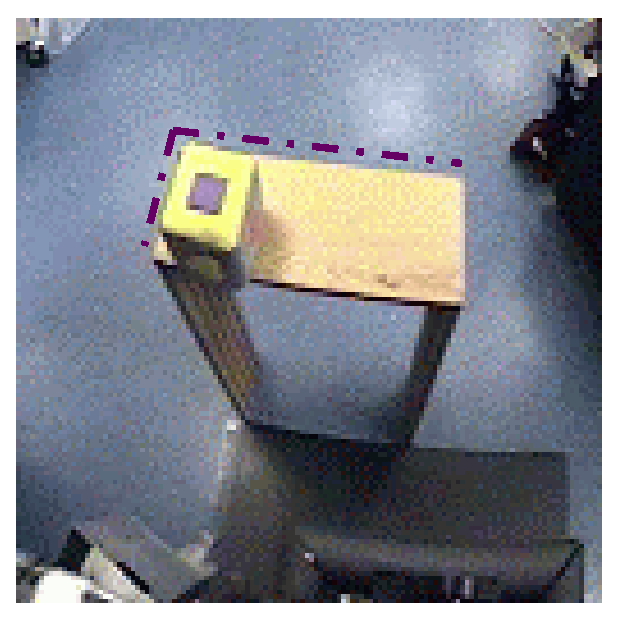
\includegraphics[width=4cm]{setup-sequence.eps}
\caption{ 
\label{fig:setup-sequence}
A cube on a table. The edges of the table and cube happen to be
aligned (dashed line), the colors of the cube and table are not well
separated, and the cube has a potentially confusing surface pattern.
}
\end{center}
\end{figure}
\fi

\ifverbose
In a robotic
implementation, the signals required
for calibrating/learning reaching can be acquired 
through a random exploration of the 
workspace~\cite{metta99developmental, Marjanovic-96-SAB}.
\fi

\ifverbose
It is not by chance that reaching has 
a sharp improvement around three months of age in sync with the
development of stereopsis \cite{}. A necessary step of these 
transformation is that of combining eye/head position signals to 
the visual position of the target. 
\fi

\ifverbose
Speaking of abilities in this on/off terms is 
perhaps too much of a clear cut and it is not a true description
of the observed infant's behavior (see for example \cite{Streri}). 
However, it helps to understand the developmental progression towards 
object manipulation. 
\fi
 


\ifverbose
NEW In this paper, we explore this link between the robot body, action,
and perception with a long-term goal of designing the architecture for
development through the natural interaction of the robot with a human
teacher. Elements of the general architecture are action and object
understanding, imitation, and ``tasking by showing''. Some behaviors
we investigated include the control of gaze (where to look), and
attentional system (what to look), and reaching (how to get the robot
effectors at manipulative distances).
\fi

\ifverbose
Neurons in area F4 are thought to provide a body map useful for
generating arm, head, and trunk movements. Our robot learns
autonomously a crude version of this body map by fusing vision and
proprioception.  As a step towards establishing the kind of visuomotor
representations seen in F5, we then develop a mechanism for using
reaching actions to visually probe the connectivity and physical
extent of objects without any prior knowledge of the appearance of the
objects (or indeed of the arm itself).
\fi

\ifverbose
The last case, that is the ``mirror neurons'' has not been implemented
yet.  We thus describe only the logic behind a possible
implementation. The logic as for the other two cases is based
extensively on the concept of causality.
\fi

\ifverbose
NEW If we had to draw a parallel with developmental neural science, we can
say we explored computationally some of the functions of the dorsal
pathway. A system similar to area F5 can provide the basis for action
and object understanding. This process of learning can be simply
initiated without necessarily solving problems such as the
object-background segregation. The exploration of object property can
situate the system favorably so to learn the criteria to be used for
segmentation later on in development.
\fi





It is interesting to consider where such
chains may lead.  In this section we briefly review the biological
literature on mirror neurons, from the point of view of what it 
would take to build them.

We explore the link between the robot body, action,
and perception with a long-term goal of designing an architecture for
development through the natural interaction of the robot with a human
teacher. Elements of the general architecture are action and object
understanding, imitation, and ``tasking by showing''. 


In this paper, we explore this link between the robot body, action,
and perception with a long-term goal of designing the architecture for
development through the natural interaction of the robot with a human
teacher. Elements of the general architecture are action and object
understanding, imitation, and ``tasking by showing''. Some behaviors
we investigated include the control of gaze (where to look), and
attentional system (what to look), and reaching (how to get the robot
effectors at manipulative distances).

The predicted position needs to be sufficiently accurate to constrain

another visual search for the exact position of the flipper.

Stereoscopic information would help further in making this
judgement.  

are likely to be diagnostic of the object's status, but more complex

Note that it is important to keep the cameras
stationary during poking.  Also, the arm detector and the poking are
not integrated.

Currently the first moving blob
to appear in the lower part of the robot's view when the reach begins
is assumed to be the arm, and the highest moving component is assumed
to be the endpoint.  Since we have control of the robot's viewpoint
and movement, they are chosen to make these assumptions likely to be
true.  



The target of a reaching operation is not assumed to be well
characterized; in fact the reaching operation serves to better define
the characteristics of the target through active segmentation
(Figure~\ref{fig:poking-sequence}).  
Hence the arm will habitually be
colliding with objects.  Sometimes the collisions will be with rigid,
more or less unyielding structures such as a table.  Sometimes the
collisions will be with movable objects the robot could potentially
manipulate.  And sometimes the collisions will be with people.  A
reaching strategy which provides useful information to the visual
system while avoiding damage to the arm or the environment will be an
important part of this work.

When trying to manipulate an unfamiliar object, it is useful to
learn something about its size, shape, orientation, weight and
physical relationship to other objects.  Motion cues, when available,
are a powerful aid in estimating such properties, since
they directly reflect the physical coherence often hidden by
misleading surface appearance.  A robot has the ability to 
actively provoke motion cues by probing the environment.
This section discusses some possible methods for doing this,
prior to actual manipulation.


The training procedure uses the open loop component of the controller,
initially containing only a few reaching points. At the end of each
reaching movement, very likely out of target, being the system
untrained at the beginning, the robot generates a self-exploratory
movement and employs the correlation algorithm. If the localization is
successful, a new training vector is available. The use of the open
loop controller guarantees with high probability that the end-point
lies within the field of view at the end of a reaching movement.

Again, this work differs from earlier approaches by being less sensitive
to distracting motion during training.  Correlated motion is also
key to poking...

is more suited to
training then actual operation, since


The arm localization is still limited: for example, in order to
maximally exploit the optic flow information, the head must be moving
very slowly when trying to locate the arm. Further, it requires the
generation of an explorative movement, which of course distracts the
robot from its task (e.g. reaching). Still, without relying on
extensive visual search, more proprioceptive information can be
employed. The idea is that of mixing positional information with the
visual detection algorithm.

A key feature of this approach is that optic flow uncorrelated with
arm motion may be ignored, so the robot is unlikely to be confused by
a distractor.

if we were able to fully model it then we
would need the Jacobian encountered before.

It turns out
that there is a different solution based on the temporal pattern of
the movement without taking into account the direction or the
amplitude - we computed the correlation over binarized versions of
both the arm velocity and the optic flow. This works for two reasons:
{\em i)} it is difficult to imagine two similar movements for a
sufficiently extended period of time, and {\em ii)} the robot, being
not a passive observer but rather the initiator of the movement can
generate a peculiar pattern which is unlikely to be encountered in the
environment.


Intuitively, this is appealing given the
human ability to adapt quickly to mirror-inverted views of their
arm, but not to latency.

There are at least two strategies that can be applied to
guide reaching by vision: open loop and closed loop. In the open loop
case the problem is that of identifying where to move the end-point in
space (by looking) and generating the appropriate sequence of motor
commands (the trajectory) to get close to the target position. It is
clear that a certain amount of open loop control is needed because the
end-point is not always within the field of view. Requiring this would
be too restrictive to the overall robot behavior. 

==========================================================================

Starting from this signature alone, and no prior information about
visual appearance, we show how a robot can locate its arm and
identify the boundaries of objects.

==========================================================================
==========================================================================



To manipulate an object, it is important to know
This property can be guessed at visually

General theme -- uniting manipulation and vision.
Specifics: poking, perceiving the manipulator itself, mirror neurons.

==================================

  If we initially imagine the object is
concave, we can track a location where the object surface is parallel
to the image plane.

We can cast pose as the relationship between the (2D) image plane and
a (2D) point on the surface of the object.

We can decompose the pose of a rigid object into the location of a
point on its surface and its orientation.  If we choose a point that
faces directly towards the camera, then there are fewer free
parameters.  Of course which particular point faces the camera varies
with time as the object rotates in depth.

   ***

When poking an object, it may be useful to track how its pose is
changing.  This is hard to do without knowing its shape.  Poking may
give us the boundary of an object, but only in the image plane.  We
would like a way to express pose that is well matched to the kind of
information we can extract.


Once we start moving objects around, by poking or otherwise, it is
useful to track their changes in pose.  Various approaches to this are
possible that ideally lead to full 3D information, such as shape from
motion, but they are by no means easy to achieve for unknown objects.
Ideally, the pose of a rigid object could be reported as a simple
six-dimensional quantity.  In reality uncertainty in the shape of the
object marshals against this.  
It would be useful to have a
representation that steps away from the appearance of the object as
little as possible.  

==========================================================================
==========================================================================


==========================================================================
==========================================================================


==========================================================================
==========================================================================



The benefits of manipulation for perception are many.  But even before
manipulation, there are many things we can do.  Simply poking things
can tell us about their shape and resolve visual ambiguities.


A big disturbance is apt to generate
  a confusing motion that is hard to process directly.  But it will
  move the object away from its local surroundings, giving another
  ``role of the dice'' -- an opportunity for the robot to see the
  object against a new background, perhaps with better contrast.
  Frequently visual ambiguity is only a local, accidental effect.

  We can use the arm's endpoint as a mobile
  reference object to confirm our theories of where free space lies.

Ask the human to present the object.  A human bringing an
object near the robot offers the dual advantage of motion cues and
a known (if complicated) partial background -- the hand.
%
One remaining alternative is to displace the robot's own head and body, again
to get another ``role of the dice'', or to access three-dimensional
information over a longer baseline than is available from the
stereo cameras.
%


==========================================================================
==========================================================================



\subsubsection*{Alternative approaches}

There are many possible approaches to head pose estimation.  At one
end of the scale, there are techniques that rely on very strong models
of head shape, such as the work of Horprasert and
Yacoob~\cite{black95tracking}.  The shape of the human head is broadly
similar across the species.  Anthropometry characterizes the
distribution of face length scales and ratios within different
sub-groups.  These distributions are quite narrow for a subject whose
gender, race, and age are known.  Horprasert and Yacoob make use of
this to estimate head orientation from monocular images.  They show
that pose can be recovered by tracking just five points on the face
(four at the eye corners and a fifth at the tip of the nose), given
that the necessary anthropometric data is available.  They propose a
two stage system that estimates a subjects gender, race and age first,
indexes into the appropriate table of anthropometric data, and then
performs the pose estimation.

At the other end of the scale, there are pose tracking systems which
do not require a prior model, and are therefore of more general
application than systems that rely on special characteristics of the
head -- for example Harville et al~\cite{harville99pose}.  

Other points on the spectrum include the application of eigenspace
techniques to directly recognize the pose of a specific user, as
opposed to tracking changes in pose~\cite{mckenna98realtime}.  And
then there are very many systems designed to run in real-time, using a
wide variety of simple cues such as hair outline~\cite{wang98hybrid}.




==========================================================================
==========================================================================


==========================================================================
==========================================================================


==========================================================================
==========================================================================




Head as simple concave object.

First, I develop a 6-dimensional coordinate system that is convenient
for tracking, deferring until later how those coordinates relate to
the rigid body parameters we really want.  The goal was to develop a
coordinate system that isolates the impact of estimates of the shape
of the head as much as possible.  In fact, the tracking scheme here
will work on concave objects of all sorts.   The
kinds of asymmetric, extended, awkwardly-shaped objects it would not
work on are exactly the kind of objects for which pose can be
determined relatively unambiguously from static images.

If an object being viewed does not rotate in depth but is otherwise
free to explore a 3D space, there are four numbers that both describe
the object's pose completely and are relatively easy to recover from
the perspective projection of the object on the image plane.  These
are~:-

\begin{itemize}

\item A position on the image plane, specified by two coordinates,
giving a ray from the camera to the object.

\item A coordinate specifying any in-plane rotation of the object,
which is the only rotational freedom it has.

\item A coordinate specifying a scaling of the projection of the
object on the image plane.

\end{itemize}

These coordinates completely describe the object's pose in the sense
that if the camera configuration is known, and {\em if the shape of
the object is known}, the full 3D pose of the object can be recovered
from these parameters.  The need for the shape of the object arises
from the implicit reference points of the coordinates -- for example,
the scaling coordinate can be converted to distance only with
knowledge of the size of the object.

\begin{figure}[tbp]
\centerline{
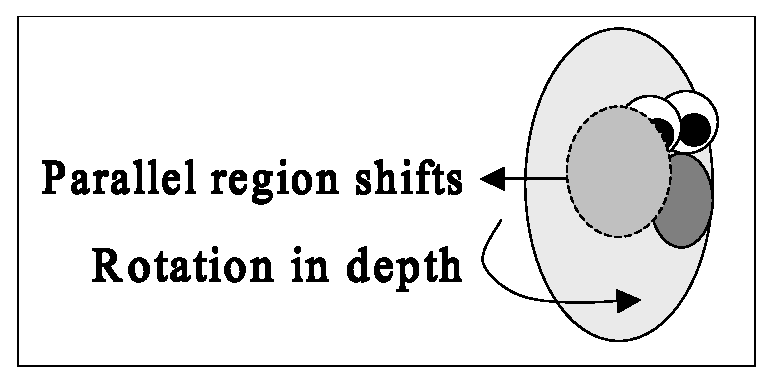
\includegraphics[width=3cm]{parallel-shift.eps}
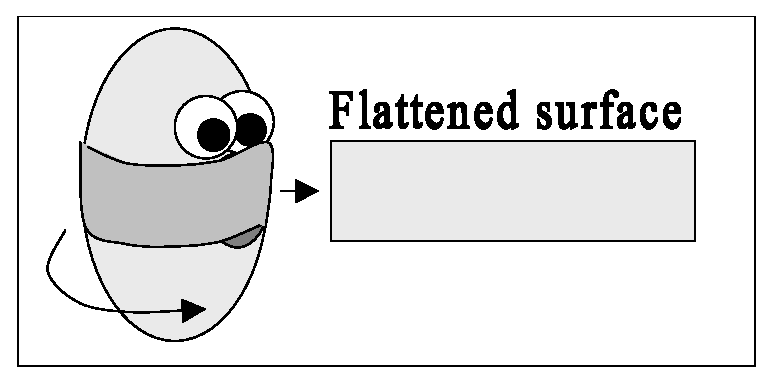
\includegraphics[width=3cm]{parallel-flat.eps}
}
\caption{ 
%
Left: when the head rotates in depth, a different region on the head
will become parallel to the image plane.  Right: if the regions of the
head that become parallel during a movement of the head do not explore
the surface in 2D, then the surface they do explore can be thought of
as Euclidean without running into contradictions (except for full
360\dgrs\ excursions).
%
}
\label{fig:parallel-shift}
\end{figure}

Once the object starts rotating in depth, there are two more degrees of
freedom to factor in.  The goal here to introduce them without
destroying the simplicity of the image plane coordinates defined
above.  Importing some domain knowledge, assume the object being
tracked is basically convex.  Then at any moment there will be a
unique region on the surface of the object that is close to parallel
to the image plane.  As the object rotates in depth, this region will
shift to another part of the surface.  We can parameterize where this
region lies on the surface of the object using two dimensions.  And
since the region is (by construction) parallel to the image plane, the
four coordinates developed earlier can be recast as follows~:-

\begin{itemize}

\item 
Two coordinates that specify where the projection of the parallel
region lies on the image plane.

\item
A coordinate specifying how the parallel region is rotated with
respect to the image plane.  This is the only rotational degree of
freedom the parallel region has, by construction.

\item 
A coordinate specifying a scaling of the parallel region (or equivalently
of the projection of the entire object, as before).

\end{itemize}

Combined with two coordinates that determine what part of the surface
of the object is currently parallel to the image plane, we have a
6-dimensional coordinate system that fully specifies the 3D pose of
the object (if the shape of the object is known).  This choice of
coordinates has some virtues.  In contrast to Euler angles, for
example, the coordinates can be considered separately and in any
order.  This is least obvious for the rotation coordinate, but becomes
clear if that coordinate is thought of as a counter-rotation of the
camera about its optical axis.

A crucial issue that has not yet been addressed is what kind of
coordinates are used to span the surface of the object being tracked.
There are many possible coordinate systems for specifying a location
on a convex surface -- for example, latitude and longitude angles.
The challenge here is to use coordinates that can be related to the
projection of the object without knowledge of its 3D shape.  There is
no such magical coordinate system, so technically at this point the
dimensions of the head have to be estimated before proceeding any
further.  But suspending disbelief for a moment, consider setting up a
Euclidean coordinate system on the surface (which can be thought of as
flattening the surface out onto a plane and then using standard
rectangular coordinates).  Of course, it isn't possible to flatten out
the surface in this way without introducing inconsistencies.  But if
we do so anyway, then coordinates on the surface of the object that
lie within the parallel region will map on to the image plane very
simply, with just a scaling and an in-plane rotation.  If we only ever
try to relate coordinates within this region, then we can relate small
steps in the image plane to small steps on the surface of the object, and
so integrate the surface coordinates without needing to know the
actual shape of the object.

The above discussion imposes two conditions~:-

\begin{enumerate}

\item We must be able to determine what part of the projection of the
object originated from a surface parallel to the image plane.

\item The path the parallel region traces across the surface of the
object must lie within a strip that is thin relative to the curvature
of the object.  The wider the strip, the less Euclidean it is.  The
strip also must not make a full 360\dgrs\ excursion, no matter how
thin it is.  

\end{enumerate}

The first condition is tractable and will be addressed shortly.  With
regard to the second condition: in practice, the estimated curvature
of the object should be factored in to the surface coordinate system,
and this becomes an argument about what kinds of movements the
accuracy of the estimate actually matters for.  The answer is as might
be expected: tracking accuracy is insensitive to the estimate of shape
for movements combining in-plane translation, scaling (translation in
depth), in-plane rotation, and rotation in depth for which all the
surface patches made successively parallel to the image plane lie
within a strip.  This includes the important case of turning away,
then turning back in an approximately symmetric manner.


To actually implement a pose tracking system based on this coordinate
system, a mesh is laid down on the projecting of the head as
illustrated in Figure~\ref{fig:mesh-init}.  Nodes on the mesh are kept
in correspondence to the face using simple template trackers, which
are destroyed if they misbehave (measured by a set of consistency
checks) and recreated elsewhere.  Scaling, in-plane rotation, and
in-plane translation are straightforward to compute from deformations
of this mesh.  As the head rotates in depth, some trackers will lose
the support of the surface they are tracking as it becomes occluded,
and so be destroyed.  New parts of the head will become visible and
have trackers assigned to their surface.

\begin{figure}[tbp]
\centerline{
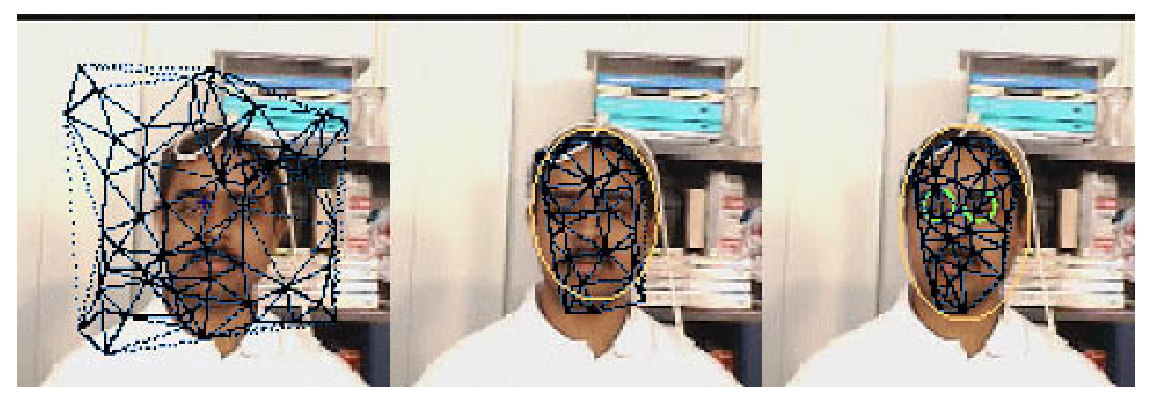
\includegraphics[width=\columnwidth]{mesh-dark-init.eps}
}
\caption{ 
%
Mesh initialization.
The mesh is initially distributed arbitrarily.  It is pruned by the
head outline when it is detected, and by heuristics based on the
relative motion of different parts of the mesh.  When frontal pose is
detected, surface coordinates of the mesh can be initialized within
the parallel region (that part of the face that is parallel to the
image plane).
%
}
\label{fig:mesh-init}
\end{figure}

The mesh is used to maintain the surface coordinate system as follows.
First, the parallel region is determined heuristically.  If the
translational component of motion can be eliminated, the parallel
region can be identified easily because the flow due to rotation peaks
there (since the motion of that surface is completely parallel
parallel to the image plane).  Translational motion can be accounted
for by normalizing flow relative to the outline of the head.  This
crude procedure works better than it should because in practice
translations and rotations of the head are often coupled so as to sum
within the parallel region rather than cancel.  Exceptions include
pure rolls and translations in depth.  The extent of the parallel
region is chosen to scale in a heuristic way with the head outline,
since in theory it should be infinitesimally small but in practice it
has to be assigned some extent to be useful.  And luckily, surface
distortions such as the nose don't seem to cause trouble.

The parallel region can be seen as a mask overlaid on the image,
within which it is safe to relate image coordinates and surface
coordinates.  Pose recognition events, detected in the manner
described in the previous section, are used to choose an origin on the
surface, and an initial translation, scaling and (in-plane) rotation
of the surface coordinate system with respect to the image plane.
This association is represented by assigning surface coordinates to
points on the mesh that lie within the parallel region, augmenting the
image plane coordinates they jointly possess.  As the parallel region
shifts during a rotation in depth, new points entering the region are
assigned surface coordinates based on their image plane coordinates,
with the transformation between the two easy to maintain using the
rotation, scaling, and translation of the mesh already recovered.

Independently of the argument given earlier for the types of movements
that can be tracked without accurate knowledge of the shape of the
head, the mesh allows a new set of trajectories to be tracked: those
which leave some portion of the face visible throughout.  The surface
coordinates of points on the mesh covering that part of the face can
be used as landmarks.

\begin{figure}[tbp]
\centerline{
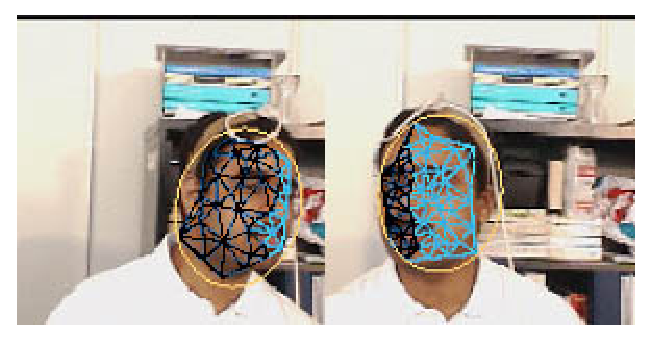
\includegraphics[width=\columnwidth]{mesh-dark-left.eps}
}
\caption{ 
%
A visualization of surface coordinates on the mesh.  The mesh has been
colored here based on the sign of a surface coordinate, so that it
appears as two halves locked onto either side of the face.
%
}
\label{fig:mesh-running}
\end{figure}


\subsubsection*{3D pose recovery}


Recovery of the 3D location of the head is straightforward, given
knowledge of the camera's parameters, although there is of course a
scale/depth ambiguity since no absolute depth information is
recovered.

Recovery of 3D orientation is equally straightforward, but shape
dependent.  The output of the tracker is effectively a procedure for
turning a specified point on the surface of the object towards the
camera and then rotating it to a specified degree.  To convert this
into Euler angles, for example, requires knowledge of the shape of the
object so that surface points can be associated with vectors from
wherever the center of the head is taken to be.  At this point, we
must make use of the estimates for the dimensions of the head from the
head tracker and make the conversion using a simple ellipsoidal model.
The crucial point is that inaccuracies in this process do not feed
back to the tracker itself.

\subsubsection*{Current results}

The system has so far been tested on a data-set made available by
Sclaroff et al~\cite{lacascia00fast}, consisting of video of head
movements with ground truth measured by a Flock of Birds sensor on the
subjects' heads.  These sequences are 200 frames in duration.  To test
the stability of the tracker over long intervals, the Sclaroff
sequences are here artificially extending by looped them forward and
back for twenty iterations.  Figure~\ref{fig:yaw-roll-result} shows
tracking results for the sequence which appeared to have the largest
rotation in depth (in no case unfortunately did the eyes become
occluded, which would have made for a better demonstration of the
advantages of the system developed in this paper).  Angular
measurements are limited by the accuracy with which they can be
initialized, which turns out to be to within about 5\dgrs\ for roll and
yaw, and about 10\dgrs\ for pitch.  Because of re-initialization
events, estimates of pose will contain discontinuities when drift is
corrected, which is not brought out in the figure.  This could be
dealt with for estimation of pose across a pre-recorded video sequence
like this one, but for use in a vision interface it seems the
discontinuities are unavoidable.  This is because the best estimate of
the current pose does truly change instantaneously when an
initialization even occurs, and there is no point propagating
information backwards to previous frames during real-time interaction
unless there is some background processing going on that can have high
latency.

\begin{figure}[tbp]
\centerline{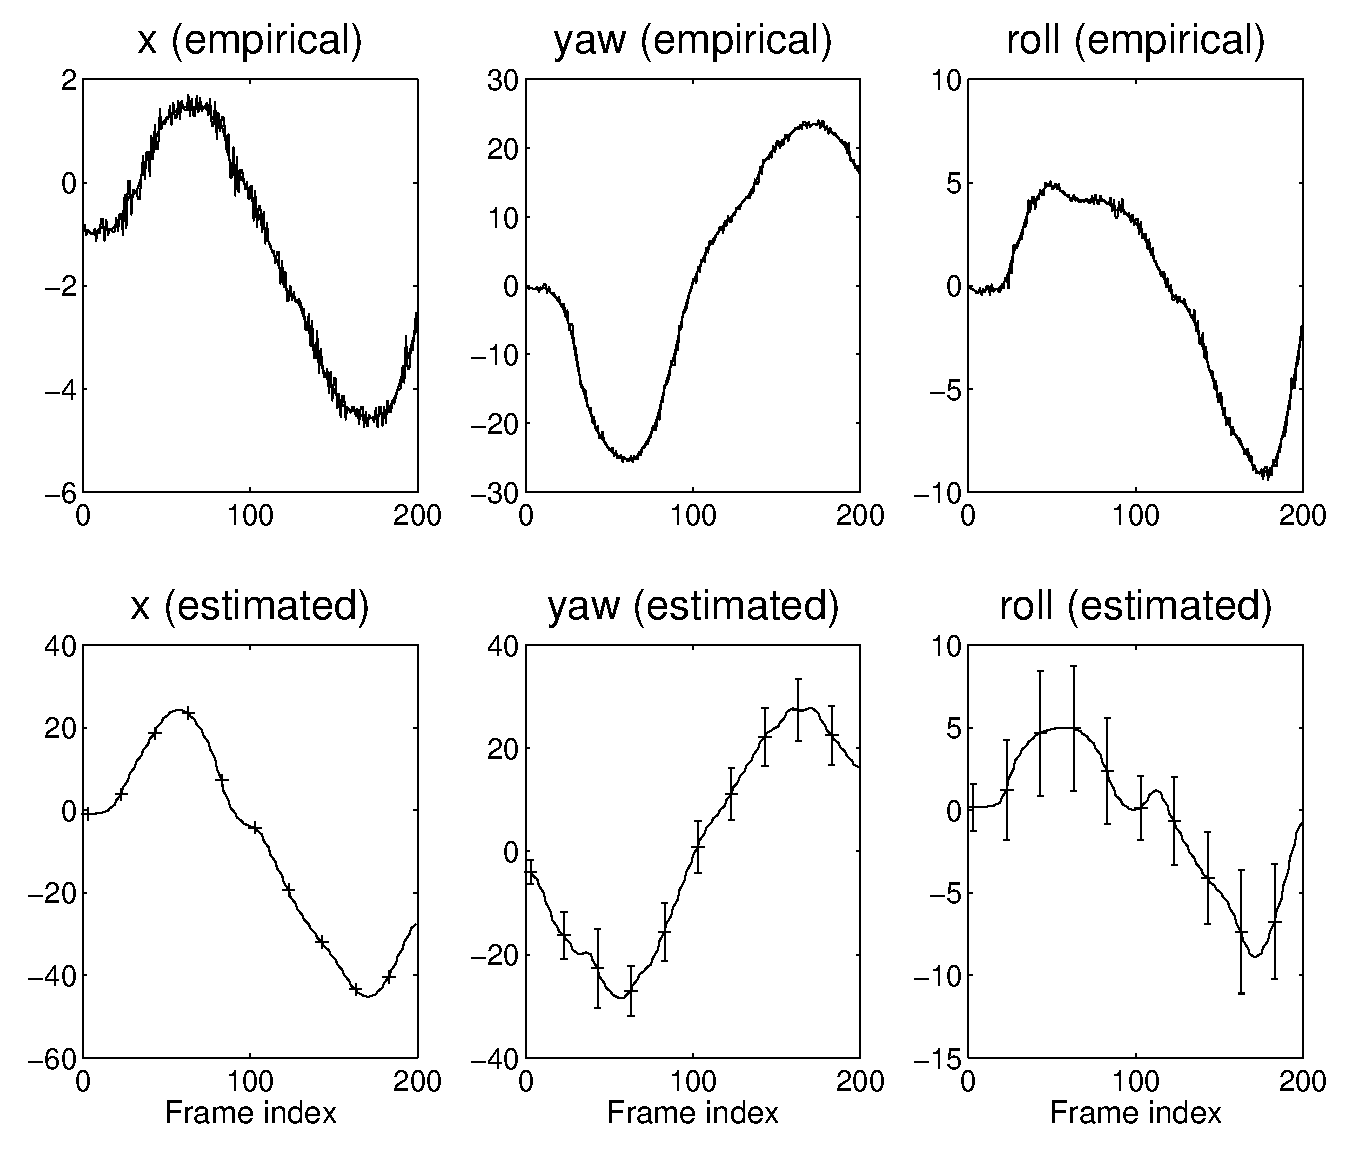
\includegraphics[width=\columnwidth]{yaw-roll-result.eps}}
\centerline{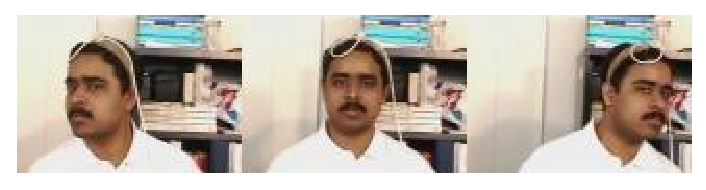
\includegraphics[width=\columnwidth]{yaw-extremes.eps}}
\caption{ 
%
Results for a sequence containing a yaw movement and horizontal
translation, with all other parameters remaining basically unchanged
except for a slight roll.  The top row shows ground truth.  The second
row shows the estimated pose parameters that change significantly
during the sequence.  The estimated $x$ coordinate is left in terms of
the image plane.  Values plotted are averaged for each
occurrence of a particular frame over a {\em single tracking run}
constructed from a sequence being played, then played in reverse, then
repeated again for twenty iterations.  Error bars show the standard
deviation of estimates for each frame.  There is about a 5\dgrs\ error
in angles, which in this case means the roll estimate is mostly noise.
%
}
\label{fig:yaw-roll-result}
\end{figure}




==========================================================================
==========================================================================


General theme -- uniting manipulation and vision.
Specifics: poking, perceiving the manipulator itself, mirror neurons.
For the purposes of manipulation, we would like to know what parts of
the environment are physically coherent ensembles -- what parts of it
will move together, and what parts are more or less independent.  This
is a difficult judgement to make from purely visual information.  This
paper looks at active strategies a robot can use to go out and gather
this information prior to manipulation.



